The following sections describe the basic inputs required for a risk
calculation, including \glspl{exposuremodel}, \glspl{fragilitymodel},
\glspl{consequencemodel}, and \glspl{vulnerabilitymodel}. In addition, each
risk calculator also requires the appropriate hazard inputs computed in the
region of interest. Hazard inputs include hazard curves for the classical
probabilistic damage and risk calculators, \gls{acr:gmf} for the scenario
damage and risk calculators, or \glspl{acr:ses} for the probabilistic event
based calculators.


\section{Exposure Models}
\label{sec:exposure}
\emph{All} risk calculators in the \glsdesc{acr:oqe} require an
\gls{exposuremodel} that needs to be provided in the \gls{acr:nrml} schema,
the use of which is illustrated through several examples in this section. The
information included in an \gls{exposuremodel} comprises a metadata section
listing general information about the exposure, followed by a cost conversions
section that describes how the different areas, costs, and occupancies for the
assets will be specified, followed by data regarding each individual
\gls{asset} in the portfolio.

A simple \gls{exposuremodel} comprising a single \gls{asset} is shown in
Listing~\ref{lst:input_exposure_minimal}.

\begin{listing}[htbp]
  \inputminted[firstline=1,firstnumber=1,fontsize=\footnotesize,frame=single,linenos,bgcolor=lightgray]{xml}{oqum/risk/verbatim/input_exposure_minimal.xml}
  \caption{Example exposure model comprising a single asset (\href{https://raw.githubusercontent.com/GEMScienceTools/oq-engine-docs/master/oqum/risk/verbatim/input_exposure_minimal.xml}{Download example})}
  \label{lst:input_exposure_minimal}
\end{listing}

Let us take a look at each of the sections in the above example file in turn.
The first part of the file contains the metadata section:

\inputminted[firstline=5,firstnumber=5,lastline=8,fontsize=\footnotesize,frame=single,linenos,bgcolor=lightgray]{xml}{oqum/risk/verbatim/input_exposure_minimal.xml}

The information in the metadata section is common to all of the \glspl{asset}
in the portfolio and needs to be incorporated at the beginning of every
\gls{exposuremodel} file. There are a number of parameters that compose the
metadata section, which is intended to provide general information regarding
the \glspl{asset} within the \gls{exposuremodel}. These parameters are
described below:

\begin{itemize}

  \item \Verb+id+: mandatory; a unique string used to identify the
    \gls{exposuremodel}. This string can contain letters~(a--z; A--Z), 
    numbers~(0--9), dashes~(--), and underscores~(\_), with a maximum of 
    100~characters.

  \item \Verb+category+: an optional string used to define the type of
    \glspl{asset} being stored (e.g: buildings, lifelines).

  \item \Verb+taxonomySource+: an optional attribute used to define the
    \gls{taxonomy} being used to classify the \glspl{asset}.

  \item \Verb+description+: mandatory; a brief string (ASCII) with further
    information about the \gls{exposuremodel}.

\end{itemize}


Next, let us look at the part of the file describing the area and cost
conversions:

\inputminted[firstline=10,firstnumber=10,lastline=15,fontsize=\footnotesize,frame=single,linenos,bgcolor=lightgray]{xml}{oqum/risk/verbatim/input_exposure_minimal.xml}

Notice that the \Verb+costType+ element defines a \Verb+name+, a \Verb+type+, 
and a \Verb+unit+ attribute.

The \gls{acr:nrml} schema for the \gls{exposuremodel} allows the definition of
a structural cost, a nonstructural components cost, a contents cost, and a
business interruption or downtime cost for each \gls{asset} in the portfolio.
Thus, the valid values for the \Verb+name+ attribute of the \Verb+costType+
element are the following:

\begin{itemize}

  \item \Verb+structural+: used to specify the structural replacement cost
    of assets

  \item \Verb+nonstructural+: used to specify the replacement cost for the
    nonstructural components of assets

  \item \Verb+contents+: used to specify the contents replacement cost

  \item \Verb+business_interruption+: used to specify the cost that will be 
    incurred per unit time that a damaged asset remains closed following an 
    earthquake

\end{itemize}

The \gls{exposuremodel} shown in the example above defines only the structural
values for the \glspl{asset}. However, multiple cost types can be defined for
each \gls{asset} in the same \gls{exposuremodel}.

The \Verb+unit+ attribute of the \Verb+costType+ element is used for
specifying the currency unit for the corresponding cost type. Note that the
\glsdesc{acr:oqe} itself is agnostic to the currency units; the \Verb+unit+ is
thus a descriptive attribute which is used by the \glsdesc{acr:oqe} to annotate the
results of a risk assessment. This attribute can be set to any valid Unicode
string.

The \Verb+type+ attribute of the \Verb+costType+ element specifies whether the
costs will be provided as an aggregated value for an asset, or per building or
unit comprising an \gls{asset}, or per unit area of an \gls{asset}. The valid
values for the \Verb+type+ attribute of the \Verb+costType+ element are the
following:

\begin{itemize}

  \item \Verb+aggregated+: indicates that the replacement costs will be 
    provided as an aggregated value for each \gls{asset}

  \item \Verb+per_asset+: indicates that the replacement costs will be 
    provided per structural unit comprising each \gls{asset}

  \item \Verb+per_area+: indicates that the replacement costs will be 
    provided per unit area for each \gls{asset}

\end{itemize}

If the costs are to be specified \Verb+per_area+ for any of the
\Verb+costTypes+, the \Verb+area+ element will also need to be defined in the
conversions section. The \Verb+area+ element defines a \Verb+type+, and a
\Verb+unit+ attribute.

The \Verb+unit+ attribute of the \Verb+area+ element is used for specifying
the units for the area of an \gls{asset}. The \glsdesc{acr:oqe} itself is
agnostic to the area units; the \Verb+unit+ is thus a descriptive attribute
which is used by the \glsdesc{acr:oqe} to annotate the results of a risk
assessment. This attribute can be set to any valid ASCII string.

The \Verb+type+ attribute of the \Verb+area+ element specifies whether the
area will be provided as an aggregated value for an \gls{asset}, or per
building or unit comprising an \gls{asset}. The valid values for the
\Verb+type+ attribute of the \Verb+area+ element are the following:

\begin{itemize}

  \item \Verb+aggregated+: indicates that the area will be provided as an 
    aggregated value for each \gls{asset}

  \item \Verb+per_asset+: indicates that the area will be provided per 
    building or unit comprising each \gls{asset}

\end{itemize}


The way the information about the characteristics of the \glspl{asset} in an
\gls{exposuremodel} are stored can vary strongly depending on how and why the
data was compiled. As an example, if national census information is used to
estimated the distribution of \glspl{asset} in a given region, it is likely
that the number of buildings within a given geographical area will be used to
define the dataset, and will be used for estimating the number of collapsed
buildings for a scenario earthquake. On the other hand, if simplified
methodologies based on proxy data such as population distribution are used to
develop the \gls{exposuremodel}, then it is likely that the built up area or
economic cost of each building typology will be directly derived, and will be
used for the estimation of economic losses.


Finally, let us look at the part of the file describing the set of
\glspl{asset} in the portfolio to be used in seismic damage or risk
calculations:

\inputminted[firstline=17,firstnumber=17,lastline=27,fontsize=\footnotesize,frame=single,linenos,bgcolor=lightgray]{xml}{oqum/risk/verbatim/input_exposure_minimal.xml}

Each \gls{asset} definition involves specifiying a set of mandatory and
optional attributes concerning the \gls{asset}. The following set of
attributes can be assigned to each \gls{asset} based on the current schema for
the \gls{exposuremodel}:

\begin{itemize}

  \item \Verb+id+: mandatory; a unique string used to identify the 
    given \gls{asset}, which is used by the \glsdesc{acr:oqe} to relate each
    \gls{asset} with its associated results. This string can contain 
    letters~(a--z; A--Z), numbers~(0--9), dashes~(-), and underscores~(\_), 
    with a maximum of 100~characters.

  \item \Verb+taxonomy+: mandatory; this string specifies the building typology
    of the given \gls{asset}. The taxonomy strings can be user-defined, or
    based on an existing classification scheme such as the GEM Taxonomy, PAGER,
    or EMS-98.

  \item \Verb+number+: the number of individual structural units comprising a
    given \gls{asset}. This attribute is mandatory for damage calculations. For
    risk calculations, this attribute must be defined if either the area or any
    of the costs are provided per structural unit comprising each \gls{asset}.

  \item \Verb+area+: area of the \gls{asset}, at a given location. As 
    mentioned earlier, the area is a mandatory attribute only if any one of the 
    costs for the \gls{asset} is specified per unit area.

  \item \Verb+location+: mandatory; specifies the longitude 
    (between -180$^{\circ}$ to 180$^{\circ}$) and latitude 
    (between -90$^{\circ}$ to 90 $^{\circ}$) of the given \gls{asset}, both
    specified in decimal degrees\footnote{Within the \glsdesc{acr:oqe}, 
    longitude and latitude coordinates are internally rounded to a precision
    of 5 digits after the decimal point.}.

  \item \Verb+costs+: specifies a set of costs for the given \gls{asset}. 
    The replacement value for different cost types must be provided on 
    separate lines within the \Verb+costs+ element. As shown in the example 
    above, each cost entry must define the \Verb+type+ and the \Verb+value+. 
    Currently supported valid options for the cost \Verb+type+ are: 
    \Verb+structural+,  \Verb+nonstructural+, \Verb+contents+, and 
    \Verb+business_interruption+.

  \item \Verb+occupancies+: mandatory only for probabilistic or scenario 
    risk calculations that specify an \Verb+occupants_vulnerability_file+.
    Each entry within this element specifies the number of
    occupants for the asset for a particular period of the day. As shown in 
    the example above, each occupancy entry must define the \Verb+period+ and 
    the \Verb+occupants+. Currently supported valid options for the 
    \Verb+period+ are: \Verb+day+, \Verb+transit+, and \Verb+night+. Currently,
    the number of \Verb+occupants+ for an asset can only be provided as an 
    aggregated value for the asset.

\end{itemize}

For the purposes of performing a retrofitting benefit/cost analysis, it is
also necessary to define the retrofitting cost (\Verb+retrofitted+). The
combination between the possible options in which these three attributes can
be defined leads to four ways of storing the information about the
\glspl{asset}. For each of these cases a brief explanation and example is
provided in this section.


\paragraph{Example 1}

This example illustrates an \gls{exposuremodel} in which the aggregated cost
(structural, nonstructural, contents and business interruption) of the
\glspl{asset} of each taxonomy for a set of locations is directly provided.
Thus, in order to indicate how the various costs will be defined, the
following information needs to be stored in the \gls{exposuremodel} file, as
shown in Listing~\ref{lst:input_exposure_cagg_metadata}.

\begin{listing}[htbp]
  \inputminted[firstline=8,firstnumber=8,lastline=18,fontsize=\footnotesize,frame=single,linenos,bgcolor=lightgray]{xml}{oqum/risk/verbatim/input_exposure_cagg.xml}
  \caption{Example exposure model using aggregate costs: metadata definition (\href{https://raw.githubusercontent.com/GEMScienceTools/oq-engine-docs/master/oqum/risk/verbatim/input_exposure_cagg.xml}{Download example})}
  \label{lst:input_exposure_cagg_metadata}
\end{listing}

In this case, the cost \Verb+type+ of each component as been defined as
\Verb+aggregated+. Once the way in which each cost is going to be defined has
been established, the values for each asset can be stored according to the
format shown in Listing~\ref{lst:input_exposure_cagg_assets}.

\begin{listing}[htbp]
  \inputminted[firstline=19,firstnumber=19,lastline=29,fontsize=\footnotesize,frame=single,linenos,bgcolor=lightgray]{xml}{oqum/risk/verbatim/input_exposure_cagg.xml}
  \caption{Example exposure model using aggregate costs: assets definition (\href{https://raw.githubusercontent.com/GEMScienceTools/oq-engine-docs/master/oqum/risk/verbatim/input_exposure_cagg.xml}{Download example})}
  \label{lst:input_exposure_cagg_assets}
\end{listing}

Each \gls{asset} is uniquely identified by its \Verb+id+. Then, a pair of
coordinates (latitude and longitude) for a \Verb+location+ where the asset is
assumed to exist is defined. Each \gls{asset} must be classified according to
a \Verb+taxonomy+, so that the \glsdesc{acr:oqe} is capable of employing the
appropriate \gls{vulnerabilityfunction} or \gls{fragilityfunction} in the risk
calculations. Finally, the cost values of each \Verb+type+ are stored within
the \Verb+costs+ attribute. In this example, the aggregated value for all
structural units (within a given \gls{asset}) at each location is provided
directly, so there is no need to define other attributes such as \Verb+number+
or \Verb+area+. This mode of representing an \gls{exposuremodel} is probably
the simplest one.


\paragraph{Example 2}

In the snippet shown in Listing~\ref{lst:input_exposure_cunit_metadata}, an
\gls{exposuremodel} containing the number of structural units and the
associated costs per unit of each \gls{asset} is presented.

\begin{listing}[htbp]
  \inputminted[firstline=8,firstnumber=8,lastline=18,fontsize=\footnotesize,frame=single,linenos,bgcolor=lightgray]{xml}{oqum/risk/verbatim/input_exposure_cunit.xml}
  \caption{Example exposure model using costs per unit: metadata definition (\href{https://raw.githubusercontent.com/GEMScienceTools/oq-engine-docs/master/oqum/risk/verbatim/input_exposure_cunit.xml}{Download example})}
  \label{lst:input_exposure_cunit_metadata}
\end{listing}

For this case, the cost \Verb+type+ has been set to \Verb+per_asset+. Then,
the information from each \gls{asset} can be stored following the format shown
in Listing~\ref{lst:input_exposure_cunit_assets}.

\begin{listing}[htbp]
  \inputminted[firstline=19,firstnumber=19,lastline=29,fontsize=\footnotesize,frame=single,linenos,bgcolor=lightgray]{xml}{oqum/risk/verbatim/input_exposure_cunit.xml}
  \caption{Example exposure model using costs per unit: assets definition (\href{https://raw.githubusercontent.com/GEMScienceTools/oq-engine-docs/master/oqum/risk/verbatim/input_exposure_cunit.xml}{Download example})}
  \label{lst:input_exposure_cunit_assets}
\end{listing}

In this example, the various costs for each \gls{asset} is not provided
directly, as in the previous example. In order to carry out the risk
calculations in which the economic cost of each \gls{asset} is provided, the
\glsdesc{acr:oqe} multiplies, for each \gls{asset}, the number of units
(buildings) by the ``per asset'' replacement cost. Note that in this case,
there is no need to specify the attribute \Verb+area+.


\paragraph{Example 3}

The example shown in Listing~\ref{lst:input_exposure_carea_aagg_metadata}
comprises an \gls{exposuremodel} containing the built up area of each
\gls{asset}, and the associated costs are provided per unit area.

\begin{listing}[htbp]
  \inputminted[firstline=8,firstnumber=8,lastline=20,fontsize=\footnotesize,frame=single,linenos,bgcolor=lightgray]{xml}{oqum/risk/verbatim/input_exposure_carea_aagg.xml}
  \caption{Example exposure model using costs per unit area and aggregated areas: metadata definition (\href{https://raw.githubusercontent.com/GEMScienceTools/oq-engine-docs/master/oqum/risk/verbatim/input_exposure_carea_aagg.xml}{Download example})}
  \label{lst:input_exposure_carea_aagg_metadata}
\end{listing}

In order to compile an \gls{exposuremodel} with this structure, the cost
\Verb+type+ should be set to \Verb+per_area+. In addition, it is also
necessary to specify if the \Verb+area+ that is being store represents the
aggregated area of number of units within an asset, or the average area of a
single unit. In this particular case, the \Verb+area+ that is being stored is
the aggregated built up area per asset, and thus this attribute was set to
\Verb+aggregated+. Listing~\ref{lst:input_exposure_carea_aagg_assets}
illustrates the definition of the \glspl{asset} for this example.

\begin{listing}[htbp]
  \inputminted[firstline=21,firstnumber=21,lastline=31,fontsize=\footnotesize,frame=single,linenos,bgcolor=lightgray]{xml}{oqum/risk/verbatim/input_exposure_carea_aagg.xml}
  \caption{Example exposure model using costs per unit area and aggregated areas: assets definition (\href{https://raw.githubusercontent.com/GEMScienceTools/oq-engine-docs/master/oqum/risk/verbatim/input_exposure_carea_aagg.xml}{Download example})}
  \label{lst:input_exposure_carea_aagg_assets}
\end{listing}

Once again, the \glsdesc{acr:oqe} needs to carry out some calculations in
order to compute the different costs per \gls{asset}. In this case, this value
is computed by multiplying the aggregated built up \Verb+area+ of each
\gls{asset} by the associated cost per unit area. Notice that in this case,
there is no need to specify the attribute \Verb+number+.


\paragraph{Example 4}

This example demonstrates an \gls{exposuremodel} that defines the number of
structural units for each \gls{asset}, the average built up area per
structural unit and the associated costs per unit area.
Listing~\ref{lst:input_exposure_carea_aunit_metadata} shows the metadata
definition for an \gls{exposuremodel} built in this manner.

\begin{listing}[htbp]
  \inputminted[firstline=8,firstnumber=8,lastline=20,fontsize=\footnotesize,frame=single,linenos,bgcolor=lightgray]{xml}{oqum/risk/verbatim/input_exposure_carea_aunit.xml}
  \caption{Example exposure model using costs per unit area and areas per unit: metadata definition (\href{https://raw.githubusercontent.com/GEMScienceTools/oq-engine-docs/master/oqum/risk/verbatim/input_exposure_carea_aunit.xml}{Download example})}
  \label{lst:input_exposure_carea_aunit_metadata}
\end{listing}

Similarly to what was described in the previous example, the various costs
\Verb+type+ also need to be established as \Verb+per_area+, but the
\Verb+type+ of area is now defined as \Verb+per_asset+.
Listing~\ref{lst:input_exposure_carea_aunit_assets} illustrates the definition
of the assets for this example.

\begin{listing}[htbp]
  \inputminted[firstline=21,firstnumber=21,lastline=31,fontsize=\footnotesize,frame=single,linenos,bgcolor=lightgray]{xml}{oqum/risk/verbatim/input_exposure_carea_aunit.xml}
  \caption{Example exposure model using costs per unit area and areas per unit: assets definition (\href{https://raw.githubusercontent.com/GEMScienceTools/oq-engine-docs/master/oqum/risk/verbatim/input_exposure_carea_aunit.xml}{Download example})}
  \label{lst:input_exposure_carea_aunit_assets}
\end{listing}

In this example, the \glsdesc{acr:oqe} will make use of all the parameters to
estimate the various costs of each \gls{asset}, by multiplying the number of
structural units by its average built up area, and then by the respective cost
per unit area.


\paragraph{Example 5}

In this example, additional information will be included, which is required
for other risk analysis besides loss estimation, such as the calculation of
insured losses or benefit/cost analysis. For the calculation of insured
losses, it is necessary to establish how the insurance \glspl{limit} and
\glspl{deductible} are going to be defined.
Listing~\ref{lst:input_exposure_ins_rel_metadata} illustrates the metadata
section of an \gls{exposuremodel} where the insurance \glspl{limit} and
\glspl{deductible} for structural components will be defined relative to the
structural replacement cost.

\begin{listing}[htbp]
  \inputminted[firstline=8,firstnumber=8,lastline=21,fontsize=\footnotesize,frame=single,linenos,bgcolor=lightgray]{xml}{oqum/risk/verbatim/input_exposure_ins_rel.xml}
  \caption{Example exposure model using relative insurance limits and deductibles: metadata definition (\href{https://raw.githubusercontent.com/GEMScienceTools/oq-engine-docs/master/oqum/risk/verbatim/input_exposure_ins_rel.xml}{Download example})}
  \label{lst:input_exposure_ins_rel_metadata}
\end{listing}

In this example, both the insurance \gls{limit} and the \gls{deductible} are
defined as a fraction of the replacement cost, by setting the attribute
\Verb+isAbsolute+ to \Verb+false+. Then, for each type of cost, the
\gls{limit} and \gls{deductible} value can be stored for each asset, as
illustrated in the snippet shown in
Listing~\ref{lst:input_exposure_ins_rel_assets}.

\begin{listing}[htbp]
  \inputminted[firstline=22,firstnumber=22,lastline=32,fontsize=\footnotesize,frame=single,linenos,bgcolor=lightgray]{xml}{oqum/risk/verbatim/input_exposure_ins_rel.xml}
  \caption{Example exposure model using relative insurance limits and deductibles: assets definition (\href{https://raw.githubusercontent.com/GEMScienceTools/oq-engine-docs/master/oqum/risk/verbatim/input_exposure_ins_rel.xml}{Download example})}
  \label{lst:input_exposure_ins_rel_assets}
\end{listing}

On the other hand, a user could define one or both of these parameters as
absolute values, by setting the aforementioned attribute to \Verb+true+. This
is shown in the example shown in Listing~\ref{lst:input_exposure_ins_abs}.

\begin{listing}[htbp]
  \inputminted[firstline=1,firstnumber=1,fontsize=\footnotesize,frame=single,linenos,bgcolor=lightgray]{xml}{oqum/risk/verbatim/input_exposure_ins_abs.xml}
  \caption{Example exposure model using absolute insurance limits and deductibles (\href{https://raw.githubusercontent.com/GEMScienceTools/oq-engine-docs/master/oqum/risk/verbatim/input_exposure_ins_abs.xml}{Download example})}
  \label{lst:input_exposure_ins_abs}
\end{listing}

Moreover, in order to perform a benefit/cost assessment, it is also necessary
to indicate the retrofitting cost. This parameter is handled in the same
manner as the structural cost, and it should be stored according to the format
shown in Listing~\ref{lst:input_exposure_retrofit}.

\begin{listing}[htbp]
  \inputminted[firstline=1,firstnumber=1,fontsize=\footnotesize,frame=single,linenos,bgcolor=lightgray]{xml}{oqum/risk/verbatim/input_exposure_retrofit.xml}
  \caption{Example exposure model specifying retrofit costs (\href{https://raw.githubusercontent.com/GEMScienceTools/oq-engine-docs/master/oqum/risk/verbatim/input_exposure_retrofit.xml}{Download example})}
  \label{lst:input_exposure_retrofit}
\end{listing}

Despite the fact that for the demonstration of how the insurance parameters
and retrofitting cost can be stored the per building type of cost structure
described in Example~1 was used, it is important to mention that any of the
other cost storing approaches can also be employed (Examples 2--4).


\paragraph{Example 6}

The \glsdesc{acr:oqe} is also capable of estimating human losses, based on the
number of occupants in an \gls{asset}, at a certain time of the day. The example
\gls{exposuremodel} shown in Listing~\ref{lst:input_exposure_occupants} illustrates
how this parameter is defined for each \gls{asset}. In addition, this example also
serves the purpose of presenting an \gls{exposuremodel} in which three cost
types have been defined using three different options.

As previously mentioned, in this example only three costs are being stored,
and each one follows a different approach. The \Verb+structural+ cost is being
defined as the aggregate replacement cost for all of the buildings comprising
the asset (Example~1), the \Verb+nonstructural+ value is defined as the
replacement cost per unit area where the area is defined per building
comprising the \gls{asset} (Example~4), and the \Verb+contents+ and
\Verb+business_interruption+ values are provided per building comprising the
\gls{asset} (Example~2). The number of occupants at different times of the day are
also provided as aggregated values for all of the buildings comprising the
\gls{asset}.

\begin{listing}[htbp]
  \inputminted[firstline=1,firstnumber=1,fontsize=\footnotesize,frame=single,linenos,bgcolor=lightgray]{xml}{oqum/risk/verbatim/input_exposure_occupants.xml}
  \caption{Example exposure model specifying the aggregate number of occupants per asset (\href{https://raw.githubusercontent.com/GEMScienceTools/oq-engine-docs/master/oqum/risk/verbatim/input_exposure_occupants.xml}{Download example})}
  \label{lst:input_exposure_occupants}
\end{listing}


A web-based tool to build an \gls{exposuremodel} in the \gls{acr:nrml} schema
are also under development, and can be found at the OpenQuake platform at the
following address: \href{https://platform.openquake.org/ipt/}{https://platform.openquake.org/ipt/}.


\section{Fragility Models}
\label{sec:fragility}
This section describes the schema currently used to store
\glspl{fragilitymodel}, which are required for the Scenario Damage Calculator
and the Classical Probabilistic Seismic Damage Calculator. In order to perform
probabilistic or scenario damage calculations, it is necessary to define a
\gls{fragilityfunction} for each building typology present in the
\gls{exposuremodel}. A \gls{fragilitymodel} defines a set of
\glspl{fragilityfunction}, describing the probability of exceeding a set of
limit, or damage, states. The \glspl{fragilityfunction} can be defined using
either a discrete or a continuous format, and the \gls{fragilitymodel} file
can include a mix of both types of \glspl{fragilityfunction}.

For discrete \glspl{fragilityfunction}, sets of probabilities of exceedance
(one set per limit state) are defined for a list of intensity measure levels,
as illustrated in Figure~\ref{fig:fragility-discrete}.

\begin{figure}[ht]
\centering
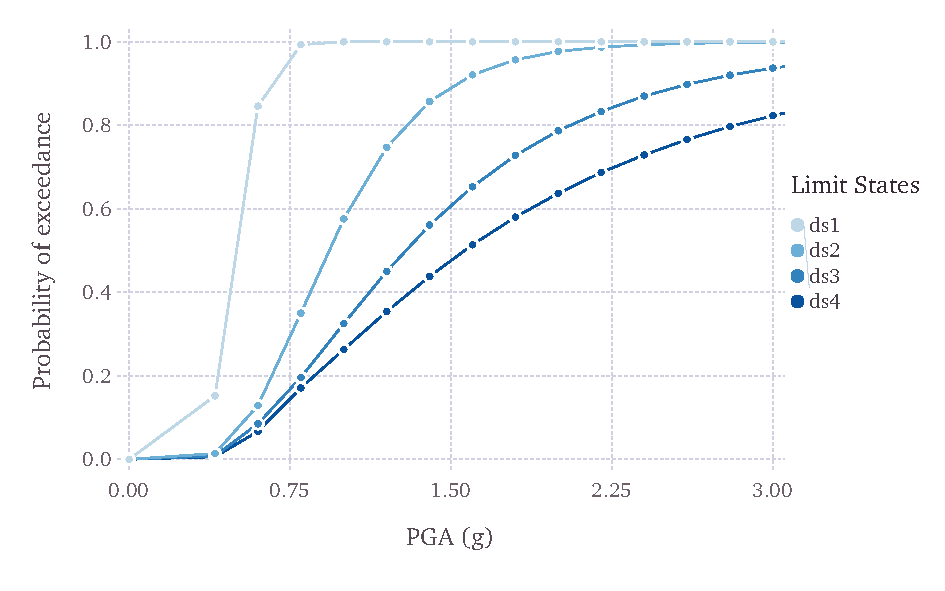
\includegraphics[width=12cm]{figures/risk/fragility-discrete.pdf}
\caption{Graphical representation of a discrete fragility model}
\label{fig:fragility-discrete}
\end{figure}

The \glspl{fragilityfunction} can also be defined as continuous functions,
through the use of cumulative lognormal distribution functions. In
Figure~\ref{fig:fragility-continuous}, a continuous \gls{fragilitymodel} is
presented.

\begin{figure}[ht]
\centering
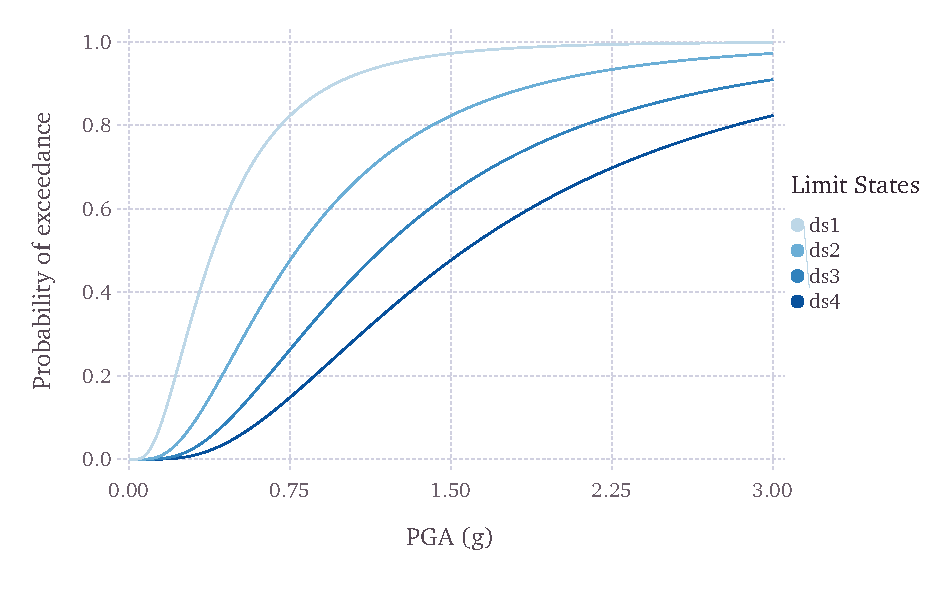
\includegraphics[width=12cm]{figures/risk/fragility-continuous.pdf}
\caption{Graphical representation of a continuous fragility model}
\label{fig:fragility-continuous}
\end{figure}

An example \gls{fragilitymodel} comprising one discrete
\gls{fragilityfunction} and one continuous \gls{fragilityfunction} is shown in
Listing~\ref{lst:input_fragility}.

\begin{listing}[htbp]
  \inputminted[firstline=1,firstnumber=1,fontsize=\footnotesize,frame=single,linenos,bgcolor=lightgray]{xml}{oqum/risk/verbatim/input_fragility.xml}
  \caption{Example fragility model comprising one discrete fragility function and one continuous fragility function (\href{https://raw.githubusercontent.com/GEMScienceTools/oq-engine-docs/master/oqum/risk/verbatim/input_fragility.xml}{Download example})}
  \label{lst:input_fragility}
\end{listing}


The initial portion of the schema contains general information that describes
some general aspects of the \gls{fragilitymodel}. The information in this
metadata section is common to all of the functions in the \gls{fragilitymodel}
and needs to be included at the beginning of every \gls{fragilitymodel} file.
The parameters of the metadata section are shown in the snippet below and
described after the snippet:

\inputminted[firstline=4,firstnumber=4,lastline=9,fontsize=\footnotesize,frame=single,linenos,bgcolor=lightgray]{xml}{oqum/risk/verbatim/input_fragility.xml}

\begin{itemize}

    \item \Verb+id+: mandatory; a unique string used to identify the 
      \gls{fragilitymodel}. This string can contain letters~(a--z; A--Z), 
      numbers~(0--9), dashes~(-), and underscores~(\_), with a maximum of 
      100~characters.

    \item \Verb+assetCategory+: an optional string used to specify the type of
      \glspl{asset} for which \glspl{fragilityfunction} will be defined in this
      file (e.g: buildings, lifelines).

    \item \Verb+lossCategory+: mandatory; valid strings for this attribute are 
      ``structural'', ``nonstructural'', ``contents'', and 
      ``business\_interruption''.

    \item \Verb+description+: mandatory; a brief string (ASCII) with further 
      relevant information about the \gls{fragilitymodel}, 
      for example, which building typologies are covered
      or the source of the functions in the \gls{fragilitymodel}.

    \item \Verb+limitStates+: mandatory; this field is used to define the number and 
      nomenclature of each limit state. Four limit states are employed in the 
      example above, but it is possible to use any number of discrete states,
      as long as a fragility curve is always defined for each limit state. The 
      limit states must be provided as a set of strings separated by whitespaces 
      between each limit state. Each limit state string can contain
      letters~(a--z; A--Z), numbers~(0--9), dashes~(-), and underscores~(\_).
      Please ensure that there is no whitespace within the name of any
      individual limit state.

\end{itemize}



The following snippet from the above \gls{fragilitymodel} example file defines a
discrete \gls{fragilityfunction}:

\inputminted[firstline=11,firstnumber=11,lastline=17,fontsize=\footnotesize,frame=single,linenos,bgcolor=lightgray]{xml}{oqum/risk/verbatim/input_fragility.xml}

The following attributes are needed to define a discrete \gls{fragilityfunction}:

\begin{itemize}

    \item \Verb+id+: mandatory; a unique string used to identify the 
      \gls{taxonomy} for which the function is being defined. This string is
      used to relate the \gls{fragilityfunction} with the relevant \gls{asset}
      in the \gls{exposuremodel}. This string can contain letters~(a--z; A--Z),
      numbers~(0--9), dashes~(-), and underscores~(\_), with a maximum of
      100~characters.

    \item \Verb+format+: mandatory; for discrete \glspl{fragilityfunction}, this
      attribute should be set to ``\Verb+discrete+''.

    \item \Verb+imls+: mandatory; this attribute specifies the list of intensity levels
      for which the limit state probabilities of exceedance will be defined. 
      In addition, it is also necessary to define the intensity measure type 
      (\Verb+imt+). Optionally, a \Verb+noDamageLimit+ can be specified, which 
      defines the intensity level below which the probability of exceedance 
      for all limit states is taken to be zero.

    \item \Verb+poes+: mandatory; this field is used to define the probabilities of 
      exceedance (\Verb+poes+) for each limit state for each discrete 
      \gls{fragilityfunction}. It is also necessary to specify which limit 
      state the exceedance probabilities are being defined for using the 
      attribute \Verb+ls+. The probabilities of exceedance for each limit state
      must be provided on a separate line; and the number of exceedance 
      probabilities for each limit state defined by the \Verb+poes+ attribute 
      must be equal to the number of intensity levels defined by the attribute 
      \Verb+imls+. Finally, the number and names of the limit states in each 
      fragility function must be equal to the number of limit states defined 
      earlier in the metadata section of the \gls{fragilitymodel} using the 
      attribute \Verb+limitStates+.

\end{itemize}



The following snippet from the above \gls{fragilitymodel} example file
defines a continuous \gls{fragilityfunction}:

\inputminted[firstline=19,firstnumber=19,lastline=25,fontsize=\footnotesize,frame=single,linenos,bgcolor=lightgray]{xml}{oqum/risk/verbatim/input_fragility.xml}

The following attributes are needed to define a continuous \gls{fragilityfunction}:

\begin{itemize}

    \item \Verb+id+: mandatory; a unique string used to identify the 
      \gls{taxonomy} for which the function is being defined. This string is
      used to relate the \gls{fragilityfunction} with the relevant \gls{asset}
      in the \gls{exposuremodel}. This string can contain letters~(a--z; A--Z),
      numbers~(0--9), dashes~(-), and underscores~(\_), with a maximum of
      100~characters.

    \item \Verb+format+: mandatory; for continuous \glspl{fragilityfunction},
      this attribute should be set to ``\Verb+continuous+''.

    \item \Verb+shape+: mandatory; for continuous \glspl{fragilityfunction}
      using the lognormal cumulative distrution, this attribute should be set
      to ``\Verb+logncdf+''. At present, only the lognormal cumulative
      distribution function can be used for representing continuous
      \glspl{fragilityfunction}.

    \item \Verb+imls+: mandatory; this element specifies aspects related to the
      intensity measure used by the the \gls{fragilityfunction}. The range of 
      intensity levels for which the continuous \glspl{fragilityfunction} are valid
      is specified using the attributes \Verb+minIML+ and \Verb+maxIML+. 
      In addition, it is also necessary to define the intensity measure type 
      \Verb+imt+. Optionally, a \Verb+noDamageLimit+ can be specified, which 
      defines the intensity level below which the probability of exceedance 
      for all limit states is taken to be zero.

    \item \Verb+params+: mandatory; this field is used to define the parameters
      of the continuous curve for each limit state for this 
      \gls{fragilityfunction}. For a lognormal cumulative distrbution function, 
      the two parameters required to specify the function are the mean and 
      standard deviation of the intensity level. These parameters are defined for 
      each limit state using the attributes \Verb+mean+ and \Verb+stddev+ 
      respectively. The attribute \Verb+ls+ specifies the limit state for which 
      the parameters are being defined. The parameters for each limit state
      must be provided on a separate line. The number and names of the limit 
      states in each \gls{fragilityfunction} must be equal to the number of limit 
      states defined earlier in the metadata section of the \gls{fragilitymodel}
      using the attribute \Verb+limitStates+.

\end{itemize}


Note that the schema for representing \glspl{fragilitymodel} has changed
between \gls{acr:nrml} v0.4 (used prior to \gls{acr:oqe17}) and \gls{acr:nrml}
v0.5 (introduced in \gls{acr:oqe17}).

A deprecation warning is printed every time you attempt to use a
\gls{fragilitymodel} in the old \gls{acr:nrml} v0.4 format in an
\gls{acr:oqe17} (or later) risk calculation. To get rid of the warning you
must upgrade the old \glspl{fragilitymodel} files to \gls{acr:nrml} v0.5. You
can use the command \Verb+upgrade_nrml+ with oq to do this as follows:

\begin{minted}[fontsize=\footnotesize,frame=single,bgcolor=lightgray]{shell-session}
user@ubuntu:~\$ oq upgrade_nrml <directory-name>
\end{minted}

The above command will upgrade all of your old \gls{fragilitymodel} files to
\gls{acr:nrml} v0.5. The original files will be kept, but with a .bak extension
appended. Notice that you will need to set the \Verb+lossCategory+ attribute
to its correct value manually. This is easy to do, since if you try to run a
computation you will get a clear error message telling the expected value for
the \Verb+lossCategory+ for each file.


Several methodologies to derive \glspl{fragilityfunction} are currently being
evaluated by \gls{acr:gem} and have been included as part of the Risk
Modeller's Toolkit, the code for which can be found on a public repository at
GitHub at the following address: 
\href{http://github.com/gemsciencetools/rmtk}{http://github.com/gemsciencetools/rmtk}.

A web-based tool to build a \gls{fragilitymodel} in the \gls{acr:nrml} schema
are also under development, and can be found at the OpenQuake platform at the
following address: \href{https://platform.openquake.org/ipt/}{https://platform.openquake.org/ipt/}.

\section{Consequence Models}
\label{sec:consequence}
Starting from \glsdesc{acr:oqe17}, the Scenario Damage calculator also accepts
\glspl{consequencemodel} in addition to \glspl{fragilitymodel}, in order to
estimate consequences based on the calculated damage distribution. The user
may provide one \gls{consequencemodel} file corresponding to each loss type
(amongst structural, nonstructural, contents, and business interruption) for
which a \gls{fragilitymodel} file is provided. Whereas providing a
\gls{fragilitymodel} file for at least one loss type is mandatory for running
a Scenario Damage calculation, providing corresponding \gls{consequencemodel}
files is optional.

This section describes the schema currently used to store
\glspl{consequencemodel}, which are optional inputs for the Scenario Damage
Calculator. A \gls{consequencemodel} defines a set of
\glspl{consequencefunction}, describing the distribution of the loss (or
consequence) ratio conditional on a set of discrete limit (or damage) states.
These \gls{consequencefunction} can be currently defined in \glsdesc{acr:oqe}
by specifying the parameters of the continuous distribution of the loss ratio
for each limit state specified in the fragility model for the corresponding
loss type, for each taxonomy defined in the exposure model.

An example \gls{consequencemodel} is shown in Listing~\ref{lst:input_consequence}.

\begin{listing}[htbp]
  \inputminted[firstline=1,firstnumber=1,fontsize=\footnotesize,frame=single,linenos,bgcolor=lightgray]{xml}{oqum/risk/verbatim/input_consequence.xml}
  \caption{Example consequence model (\href{https://raw.githubusercontent.com/GEMScienceTools/oq-engine-docs/master/oqum/risk/verbatim/input_consequence.xml}{Download example})}
  \label{lst:input_consequence}
\end{listing}	

The initial portion of the schema contains general information that describes
some general aspects of the \gls{consequencemodel}. The information in this
metadata section is common to all of the functions in the
\gls{consequencemodel} and needs to be included at the beginning of every
\gls{consequencemodel} file. The parameters are described below:

\begin{itemize}

  \item \Verb+id+: a unique string used to identify the \gls{consequencemodel}.
    This string can contain letters~(a--z; A--Z), numbers~(0--9), dashes~(-), 
    and underscores~(\_), with a maximum of 100~characters.

  \item \Verb+assetCategory+: an optional string used to specify the type of
    \glspl{asset} for which \glspl{consequencefunction} will be defined in
    this file (e.g: buildings, lifelines).

  \item \Verb+lossCategory+: mandatory; valid strings for this attribute are 
    ``structural'', ``nonstructural'', ``contents'', and 
    ``business\_interruption''.

  \item \Verb+description+: mandatory; a brief string (ASCII) with further 
    information about the \gls{consequencemodel}, for example, which building
    typologies are covered or the source of the functions in the
    \gls{consequencemodel}.

  \item \Verb+limitStates+: mandatory; this field is used to define the number and 
    nomenclature of each limit state. Four limit states are employed in the 
    example above, but it is possible to use any number of discrete states. The 
    limit states must be provided as a set of strings separated by whitespaces 
    between each limit state. Each limit state string can contain
    letters~(a--z; A--Z), numbers~(0--9), dashes~(-), and underscores~(\_). 
    Please ensure that there is no whitespace within the name of any individual
    limit state. The number and nomenclature of the limit states used in the
    \gls{consequencemodel} should match those used in the corresponding
    \gls{fragilitymodel}.

\end{itemize}

\inputminted[firstline=4,firstnumber=4,lastline=9,fontsize=\footnotesize,frame=single,linenos,bgcolor=lightgray]{xml}{oqum/risk/verbatim/input_consequence.xml}

The following snippet from the above \gls{consequencemodel} example file
defines a \gls{consequencefunction} using a lognormal distribution to model
the uncertainty in the consequence ratio for each limit state:

\inputminted[firstline=11,firstnumber=11,lastline=16,fontsize=\footnotesize,frame=single,linenos,bgcolor=lightgray]{xml}{oqum/risk/verbatim/input_consequence.xml}

The following attributes are needed to define a \gls{consequencefunction}:

\begin{itemize}

  \item \Verb+id+: mandatory; a unique string used to identify the 
    \gls{taxonomy} for which the function is being defined. This string is used
    to relate the \gls{consequencefunction} with the relevant \gls{asset} in the 
    \gls{exposuremodel}. This string can contain letters~(a--z; A--Z),
    numbers~(0--9), dashes~(-), and underscores~(\_), with a maximum of
    100~characters.

  \item \Verb+dist+: mandatory; for vulnerability function which use a continuous 
    distribution to model the uncertainty in the conditional loss ratios, 
    this attribute should be set to either ``\Verb+LN+'' if using the lognormal
    distribution, or to ``\Verb+BT+'' if using the Beta distribution
    \footnote{Note that as of \glsdesc{acr:oqe18}, the uncertainty in the 
    consequence ratios is ignored, and only the mean consequence ratios for the
    set of limit states is considered when computing the consequences from the
    damage distribution. Consideration of the uncertainty in the consequence
    ratios is planned for future releases of the \glsdesc{acr:oqe}.}.

  \item \Verb+params+: mandatory; this field is used to define the parameters of 
    the continuous distribution used for modelling the uncertainty in the
    loss ratios for each limit state for this 
    \gls{consequencefunction}. For a lognormal distrbution, 
    the two parameters required to specify the function are the mean and 
    standard deviation of the consequence ratio. These parameters are defined for 
    each limit state using the attributes \Verb+mean+ and \Verb+stddev+ 
    respectively. The attribute \Verb+ls+ specifies the limit state for which 
    the parameters are being defined. The parameters for each limit state
    must be provided on a separate line. The number and names of the limit 
    states in each \gls{consequencefunction} must be equal to the number of limit 
    states defined in the corresponding \gls{fragilitymodel}
    using the attribute \Verb+limitStates+.

\end{itemize}

\section{Vulnerability Models}
\label{sec:vulnerability}
In order to perform probabilistic or scenario risk calculations, it is
necessary to define a \gls{vulnerabilityfunction} for each building typology
present in the \gls{exposuremodel}. In this section, the schema for the
\gls{vulnerabilitymodel} is described in detail. A graphical representation of
a \gls{vulnerabilitymodel} (mean loss ratio for a set of intensity measure
levels) is illustrated in Figure~\ref{fig:vulnerability-zero-cov}.

\begin{figure}[ht]
\centering
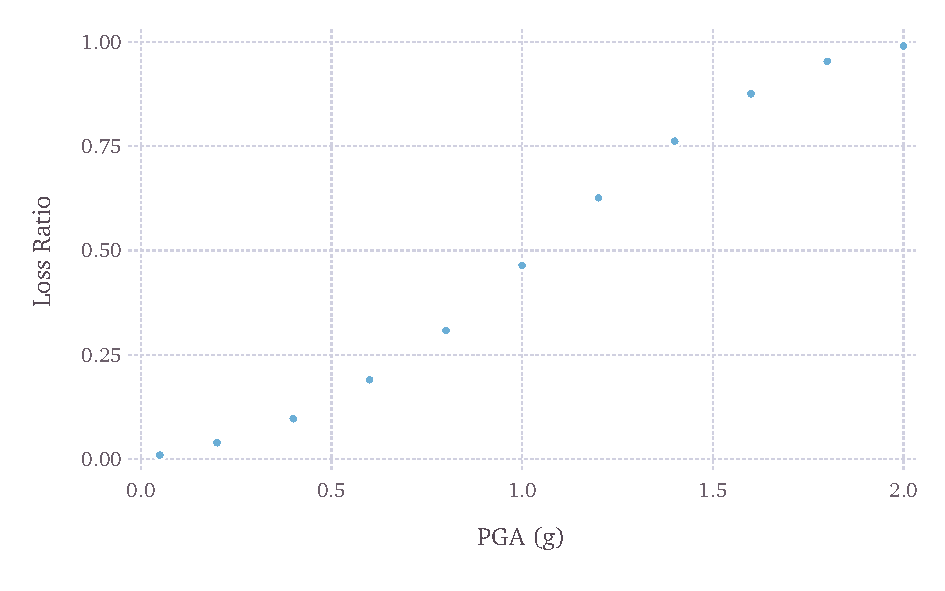
\includegraphics[width=12cm]{figures/risk/vulnerability-zero-cov.pdf}
\caption{Graphical representation of a vulnerability model}
\label{fig:vulnerability-zero-cov}
\end{figure}


Note that although the uncertainty for each loss ratio is not represented in
Figure~\ref{fig:vulnerability-zero-cov}, it can be considered in the input
file, by means of a coefficient of variation per loss ratio and a
probabilistic distribution, which can currently be set to lognormal~(LN),
Beta~(BT); or by specifying a discrete probability mass~(PM)\footnote{As of
\glsdesc{acr:oqe18}, the ``PM'' option for defining
\glspl{vulnerabilityfunction} is supported by the Scenario Risk and the
Stochastic Event-Based Probabilistic Risk Calculators, but not by the
Classical Probabilistic Risk Calculator.} distribution of the loss ratio at a
set of intensity levels. An example of a \gls{vulnerabilityfunction} that
models the uncertainty in the loss ratio at different intensity levels using a
lognormal distribution is illustrated in 
Figure~\ref{fig:vulnerability-nonzero-cov}.

\begin{figure}[ht]
\centering
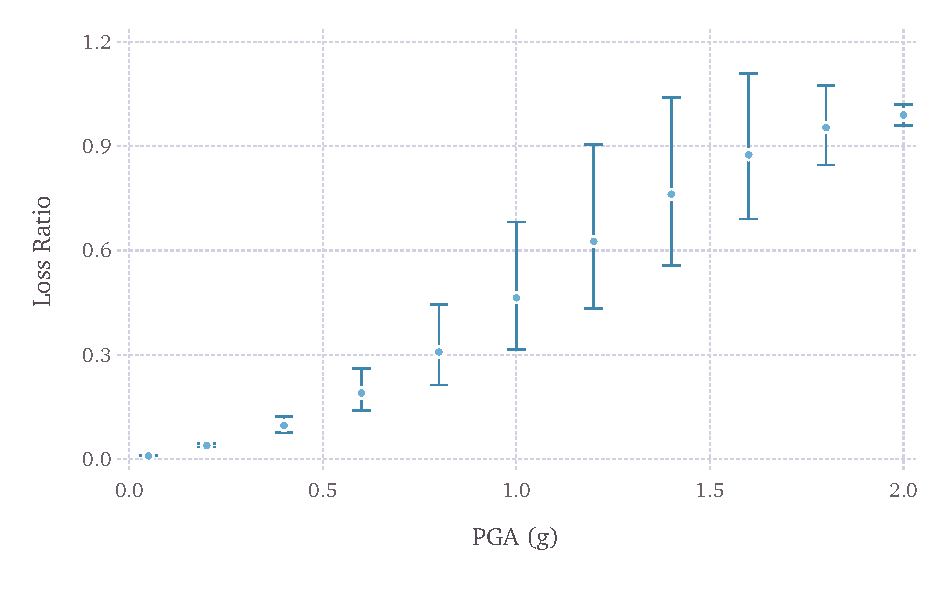
\includegraphics[width=12cm]{figures/risk/vulnerability-nonzero-cov.pdf}
\caption{Graphical representation of a vulnerability function that models the uncertainty in the loss ratio using a lognormal distribution. The mean loss ratios and coefficients of variation are illustrated for a set of intensity levels.}
\label{fig:vulnerability-nonzero-cov}
\end{figure}

In general, defining \glspl{vulnerabilityfunction} requires the user to
specify the distribution of the loss ratio for a set of intensity levels. The
loss ratio distributions can be defined using either a discrete or a
continuous format, and the \gls{vulnerabilitymodel} file can include a mix of
both types of \glspl{vulnerabilityfunction}. It is also possible to define a
\gls{vulnerabilityfunction} using a set of deterministic loss ratios
corresponding to a set of intensity levels (i.e., ignoring the uncertainty in
the conditional loss ratios).

An example \gls{vulnerabilitymodel} comprising three
\glspl{vulnerabilityfunction} is shown in
Listing~\ref{lst:input_vulnerability}. This \gls{vulnerabilitymodel} contains
one function that uses the lognormal distribution to represent the uncertainty
in the loss ratio at different intensity levels, one function that uses the
Beta distribution, and one function that is defined using a discrete
probability mass distribution.

\begin{listing}[htbp]
  \inputminted[firstline=1,firstnumber=1,fontsize=\footnotesize,frame=single,linenos,bgcolor=lightgray]{xml}{oqum/risk/verbatim/input_vulnerability.xml}
  \caption{Example vulnerability model (\href{https://raw.githubusercontent.com/GEMScienceTools/oq-engine-docs/master/oqum/risk/verbatim/input_vulnerability.xml}{Download example})}
  \label{lst:input_vulnerability}
\end{listing}


The initial portion of the schema contains general information that describes
some general aspects of the \gls{vulnerabilitymodel}. The information in this
metadata section is common to all of the functions in the
\gls{vulnerabilitymodel} and needs to be included at the beginning of every
\gls{vulnerabilitymodel} file. The parameters are illustrated in the snippet
shown and described below:

\inputminted[firstline=4,firstnumber=4,lastline=8,fontsize=\footnotesize,frame=single,linenos,bgcolor=lightgray]{xml}{oqum/risk/verbatim/input_vulnerability.xml}

\begin{itemize}

  \item \Verb+id+: a unique string (ASCII) used to identify the
    \gls{vulnerabilitymodel}. This string can contain letters~(a--z; A--Z),
    numbers~(0--9), dashes~(-), and underscores~(\_), with a maximum of
    100~characters.

  \item \Verb+assetCategory+: an optional string (ASCII) used to specify the
    type of \glspl{asset} for which \glspl{vulnerabilityfunction} will be 
    defined in this file (e.g: buildings, lifelines).

  \item \Verb+lossCategory+: mandatory; valid strings for this attribute are 
    ``structural'', ``nonstructural'', ``contents'',  
    ``business\_interruption'', and ``occupants''.

  \item \Verb+description+: mandatory; a brief string with further information about the
    \gls{vulnerabilitymodel}, for example, which building typologies are 
    covered or the source of the functions in the \gls{vulnerabilitymodel}.

\end{itemize}


The following snippet from the above \gls{vulnerabilitymodel} example file defines
a \gls{vulnerabilityfunction} modelling the uncertainty in the conditional loss
ratios using a (continuous) lognormal distribution:

\inputminted[firstline=10,firstnumber=10,lastline=14,fontsize=\footnotesize,frame=single,linenos,bgcolor=lightgray]{xml}{oqum/risk/verbatim/input_vulnerability.xml}

The following attributes are needed to define a \gls{vulnerabilityfunction} which
uses a continuous distribution to model the uncertainty in the conditional
loss ratios:

\begin{itemize}

  \item \Verb+id+: a unique string (ASCII) used to identify the \gls{taxonomy} for 
    which the function is being defined. This string is used to relate the 
    \gls{vulnerabilityfunction} with the relevant \gls{asset} in the 
    \gls{exposuremodel}. This string can contain letters~(a--z; A--Z), 
    numbers~(0--9), dashes~(-), and underscores~(\_), with a maximum of
    100~characters.

  \item \Verb+dist+: mandatory; for \glspl{vulnerabilityfunction} which use a continuous 
    distribution to model the uncertainty in the conditional loss ratios, 
    this attribute should be set to either ``\Verb+LN+'' if using the lognormal
    distribution, or to ``\Verb+BT+'' if using the Beta distribution.

  \item \Verb+imls+: mandatory; this attribute specifies the list of intensity levels
    for which the parameters of the conditional loss ratio distributions will
    be defined. In addition, it is also necessary to define the intensity 
    measure type (\Verb+imt+).

  \item \Verb+meanLRs+: mandatory; this field is used to define the mean loss ratios
    for this \gls{vulnerabilityfunction} for each of the intensity levels
    defined by the attribute \Verb+imls+. The number of mean loss ratios
    defined by the \Verb+meanLRs+ attribute must be equal to the number of
    intensity levels defined by the attribute \Verb+imls+.

  \item \Verb+covLRs+: mandatory; this field is used to define the coefficient of 
    variation for the conditional distribution of the loss ratios for this
    \gls{vulnerabilityfunction} for each of the intensity levels defined by
    the attribute \Verb+imls+. The number of coefficients of variation of loss
    ratios defined by the \Verb+covLRs+ attribute must be equal to the number
    of intensity levels defined by the attribute \Verb+imls+. The uncertainty
    in the conditional loss ratios can be ignored by setting all of the
    \Verb+covLRs+ for a given \gls{vulnerabilityfunction} to zero.

\end{itemize}


The next snippet from the \gls{vulnerabilitymodel} example file of
Listing~\ref{lst:input_vulnerability} defines a \gls{vulnerabilityfunction}
which models the uncertainty in the conditional loss ratios using a
(discrete) probability mass distribution:

\inputminted[firstline=24,firstnumber=24,lastline=33,fontsize=\footnotesize,frame=single,linenos,bgcolor=lightgray]{xml}{oqum/risk/verbatim/input_vulnerability.xml}

The following attributes are needed to define a \gls{vulnerabilityfunction}
which uses a discrete probability mass distribution to model the uncertainty
in the conditional loss ratios:

\begin{itemize}

  \item \Verb+id+: a unique string (ASCII) used to identify the \gls{taxonomy} for 
    which the function is being defined. This string is used to relate the 
    \gls{vulnerabilityfunction} with the relevant \gls{asset} in the 
    \gls{exposuremodel}. This string can contain letters~(a--z; A--Z), 
    numbers~(0--9), dashes~(-), and underscores~(\_), with a maximum of
    100~characters.

  \item \Verb+dist+: mandatory; for \glspl{vulnerabilityfunction} which use a 
    discrete probability mass distribution to model the uncertainty in the
    conditional loss ratios, this attribute should be set to ``\Verb+PM+''.

  \item \Verb+imls+: mandatory; this attribute specifies the list of intensity levels
    for which the parameters of the conditional loss ratio distributions will
    be defined. In addition, it is also necessary to define the intensity 
    measure type (\Verb+imt+).

  \item \Verb+probabilities+: mandatory; this field is used to define the
    probability of observing a particular loss ratio (specified for each row of
    \Verb+probabilities+ using the attribute \Verb+lr+), conditional on the set
    of intensity levels specified using the attribute \Verb+imls+.
    for this \gls{vulnerabilityfunction}. Thus, the number of probabilities
    defined by each \Verb+probabilities+ attribute must be equal to the number
    of intensity levels defined by the attribute \Verb+imls+. On the other hand,
    there is no limit to the number of loss ratios for which
    \Verb+probabilities+ can be defined. In the example shown here, notice that
    the set of probabilities conditional on any particular intensity level,
    say, $MMI = 8$, sum up to one.

\end{itemize}


Note that the schema for representing \glspl{vulnerabilitymodel} has changed
between \gls{acr:nrml} v0.4 (used prior to \gls{acr:oqe17}) and \gls{acr:nrml}
v0.5 (introduced in \gls{acr:oqe17}).

A deprecation warning is printed every time you attempt to use a
\gls{vulnerabilitymodel} in the old \gls{acr:nrml} v0.4 format in an
\gls{acr:oqe17} (or later) risk calculation. To get rid of the warning you
must upgrade the old \glspl{vulnerabilitymodel} files to \gls{acr:nrml} v0.5.
You can use the command \Verb+upgrade_nrml+ with oq to do this as
follows:

\begin{minted}[fontsize=\footnotesize,frame=single,bgcolor=lightgray]{shell-session}
user@ubuntu:~\$ oq upgrade_nrml <directory-name>
\end{minted}

The above command will upgrade all of your old \gls{vulnerabilitymodel} files to
\gls{acr:nrml} v0.5. The original files will be kept, but with a .bak extension
appended. Notice that you will need to set the \Verb+lossCategory+ attribute
to its correct value manually. This is easy to do, since if you try to run a
computation you will get a clear error message telling the expected value for
the \Verb+lossCategory+ for each file.


Several methodologies to derive \glspl{vulnerabilityfunction} are currently being
evaluated by \gls{acr:gem} and have been included as part of the Risk
Modeller's Toolkit, the code for which can be found on a public repository at
GitHub at: 
\href{http://github.com/gemsciencetools/rmtk}{http://github.com/gemsciencetools/rmtk}.

A web-based tool to build an \gls{vulnerabilitymodel} in the \gls{acr:nrml} schema
are also under development, and can be found at the OpenQuake platform at the
following address: \href{https://platform.openquake.org/ipt/}{https://platform.openquake.org/ipt/}.
